\documentclass[11pt,a4paper]{article}
\usepackage[margin=2.3cm]{geometry}
\usepackage[T1]{fontenc}
\usepackage{lmodern,microtype,amsmath,amssymb,booktabs,graphicx,xcolor,enumitem,siunitx}
\usepackage[font=small,labelfont=bf]{caption}
\usepackage{tikz}
\usetikzlibrary{arrows.meta,positioning,fit,calc}
\usepackage[numbers,sort&compress]{natbib}
\usepackage[colorlinks=true,linkcolor=blue!50!black,citecolor=green!35!black,urlcolor=blue!50!black]{hyperref}

\definecolor{sens}{HTML}{D64545}
\definecolor{motl}{HTML}{2E8B57}
\definecolor{motr}{HTML}{2F6FD0}
\newcommand{\code}[1]{\texttt{#1}}
\newcommand{\todo}{\item[$\square$]}
\newcommand{\done}{\item[$\boxtimes$]}

\title{Steering through a scanned living room with a dish of neurons\\[0.3em]
\large A closed-loop navigation experiment for the Cortical Labs CL1}
\author{Alara Dirik}
\date{Outlier Labs Biocomputing Hack, November 2026 \quad (working notes)}

\begin{document}
\maketitle

\begin{abstract}
\noindent DishBrain showed that cortical cultures on a multi-electrode array improve at Pong when
the ball's position is delivered as electrical stimulation and the outcome of each rally is fed
back as either predictable or unpredictable stimulation~\citep{kagan2022dishbrain}. This document
describes a closed-loop experiment that takes the same idea from a one-dimensional paddle to
navigation in a real 3D scene. A disc-shaped agent drives at constant speed through the ICL-NUIM
living room, a synthetic indoor scene distributed as a point cloud~\citep{handa2014iclnuim,choi2015robust}.
The point cloud is converted into an obstacle map, from which eight range rays are cast around
the agent. Each ray's distance sets the pulse rate (\SIrange{4}{40}{\hertz}) on one of eight
sensory electrodes of the CL1's $8\times8$ array. Spiking in two motor regions at the edges of
the array turns the agent left or right. Progress towards the goal and reaching it earn
predictable stimulation; collisions earn four seconds of unpredictable stimulation. The
experiment includes the silent-feedback and rest controls from DishBrain, a mirrored-layout
control, and a toy culture for the cl-sdk simulator that tests the whole encode--decode chain
before any cells are involved. On the simulator, a toy culture wired as a Braitenberg avoider
steers away from walls (steering coupling $r\approx-0.5$) and gets about six times further along
the route than a toy culture whose responses never reach the motor regions. Neither shows a
trend across episodes, which is correct because the toy culture cannot learn. The checks also
caught a decoder design that produced spurious ``learning'' on this non-plastic culture. No
results on living cells are reported yet.
\end{abstract}

\section{Introduction}

Biological neural networks learn from very few samples and use little energy, which has
renewed interest in using living neurons as computing substrates~\citep{smirnova2022pong}. The
Cortical Labs CL1 makes this experiment programmable. Neurons grow on a 64-electrode array, and
a Python API (\code{cl}) reads detected spikes and schedules current-controlled stimulation in a
loop that runs at up to \SI{25}{\kilo\hertz}~\citep{clapidoc,clsdk}. In principle, anyone who
can write a game loop can embody a culture.

The best-known embodied culture is DishBrain~\citep{kagan2022dishbrain}. The ball's position
was place- and rate-coded onto eight sensory electrodes, spikes in predefined motor regions
moved the paddle, and each hit was followed by a predictable stimulus while each miss was
followed by an unpredictable one. Cultures given this feedback improved within a session;
cultures given no feedback or no sensory input did not improve in the same way. The design is
motivated by the free-energy principle~\citep{friston2010fep}: a network that can act on its
inputs should come to avoid the actions that lead to unpredictable stimulation.

Pong is a one-dimensional control problem with a dense reward. This project asks the next
question on a hackathon timescale: \emph{does the same closed loop work when the world is a real
3D scene and the task is navigation?} Navigation is harder in three ways. The input describes a
2D layout rather than one coordinate. A good action depends on obstacles all around the agent.
And the goal is out of sight, so reward comes only through feedback about progress.

The deliverable is a complete, runnable pipeline rather than a result:
\begin{itemize}[nosep]
  \item a scene converter that turns the ICL-NUIM point cloud into an obstacle grid, a drivable
        grid and a geodesic distance field (\code{prepare\_scene.py});
  \item a closed loop for the CL1 with a DishBrain-style encoder, a baseline-normalised
        decoder and a feedback state machine with three conditions (\code{run.py}, \code{world.py});
  \item a toy culture for the cl-sdk simulator that responds to stimulation, giving a positive
        and a negative control for the pipeline (\code{culture.py});
  \item analysis of outcomes, within-session learning, condition differences, sensorimotor
        coupling and stimulation artifacts (\code{analyze.py}), and a live view
        (\code{visualiser/}).
\end{itemize}

\section{Related work}

\paragraph{Embodied cultures.} Closing the loop between a cultured network and a body is older
than the CL1. In the neurally controlled animat, activity in a rat cortical culture moved a
simulated animal, and the animal's movement was fed back as stimulation~\citep{demarse2001animat}.
\citet{novellino2007robot} connected cultures to a wheeled robot: left and right infrared sensors
were rate-coded onto stimulation, and firing in two groups of electrodes set the two wheel speeds,
producing obstacle avoidance. This is the closest precedent for the sensor layout used here.
\citet{chao2008shaping} trained an embodied culture towards goal-directed movement with
patterned training stimulation chosen by a feedback controller, and \citet{warwick2010robot} drove
a mobile robot from a culture. These systems mostly relied on a hand-designed sensorimotor
mapping or explicit training stimulation, not on predictable versus unpredictable feedback.

\paragraph{Learning from structured feedback.} \citet{shahaf2001learning} showed that cultures
can learn a stimulus--response mapping when stimulation stops as soon as the desired response
appears, and \citet{isomura2015bss} showed that cultured networks separate mixed sources in a way
consistent with free-energy minimisation. DishBrain combined these ideas in a game: predictable
stimulation after a hit, unpredictable stimulation after a miss~\citep{kagan2022dishbrain}. A
follow-up compared the cultures with deep reinforcement learning agents given the same number of
episodes and found the cultures more sample efficient~\citep{khajehnejad2024sample}. Most
recently, \citet{robbins2026organoids} embodied cortical organoids in the cart-pole task. They
delivered a training signal only when performance stopped improving, chose which electrodes
received it with a reinforcement learning algorithm, and found that this adaptive training
clearly outperformed random training. The improvement was short-lived: it had faded after
45 minutes of rest.

\paragraph{Cultures as reservoirs.} A different line of work treats the culture as a fixed
nonlinear system and trains only a readout: Brainoware used an organoid to recognise speakers
from audio~\citep{cai2023brainoware}. On the CL1, \citet{loeffler2026digits} classified
spatio-temporal MNIST digits with human iPSC-derived cultures. They found that modular cortical
networks did best, and that without strict artifact control and trial-based cross-validation,
stimulation artifacts and temporal leakage can produce false positives. This experiment adopts
two lessons from that work: motor electrodes are physically separated from stimulated ones, and
the analysis checks directly whether stimulation reaches the motor electrodes
(Section~\ref{sec:analysis}).

\paragraph{The scene.} ICL-NUIM is a synthetic living room and office built for benchmarking RGB-D
odometry and reconstruction~\citep{handa2014iclnuim}; the augmented version distributed with
Open3D~\citep{choi2015robust,zhou2018open3d} includes a dense point cloud of the room, which is
used here.

\section{Method}

\begin{figure}[t]
\centering
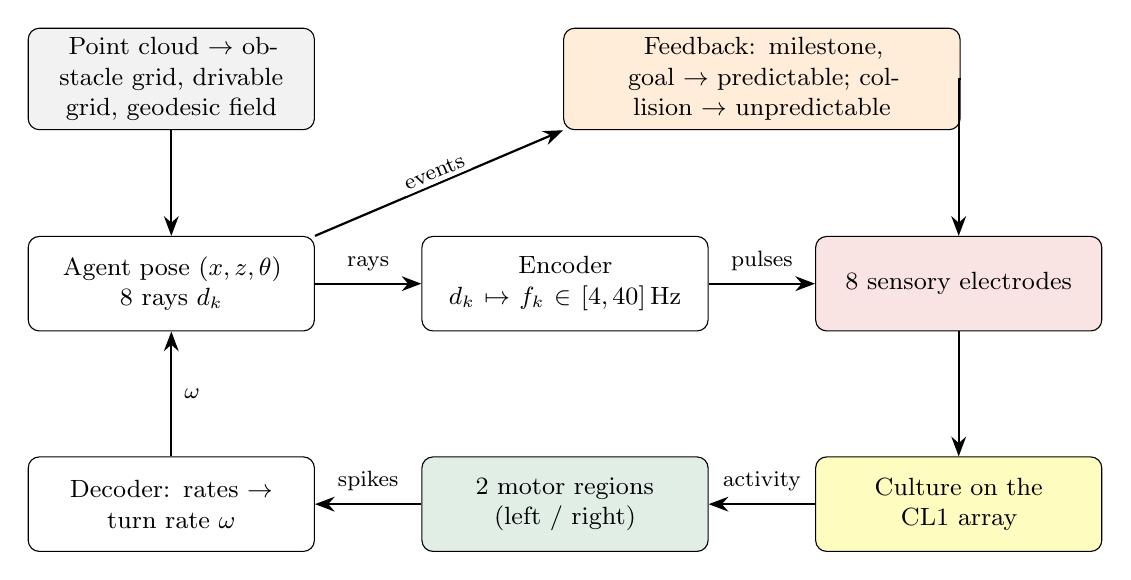
\begin{tikzpicture}[box/.style={draw, rounded corners, align=center, font=\small,
  minimum height=12mm, text width=34mm, fill=#1}, box/.default=white,
  arr/.style={-{Stealth[length=2.5mm]}, thick}, lab/.style={font=\footnotesize, fill=white, inner sep=1.5pt}]
  \node[box=gray!10] (scene) at (0, 2.6) {Point cloud $\to$ obstacle grid, drivable grid, geodesic field};
  \node[box]         (agent) at (0, 0)   {Agent pose $(x,z,\theta)$\\ 8 rays $d_k$};
  \node[box]         (enc)   at (5, 0)   {Encoder\\ $d_k\mapsto f_k\in[4,40]$\,Hz};
  \node[box=sens!15] (sens)  at (10, 0)  {8 sensory electrodes};
  \node[box=yellow!25] (cult) at (10, -2.8) {Culture on the\\ CL1 array};
  \node[box=motl!15] (mot)   at (5, -2.8) {2 motor regions\\ (left / right)};
  \node[box]         (dec)   at (0, -2.8) {Decoder: rates $\to$\\ turn rate $\omega$};
  \node[box=orange!15, text width=48mm] (fb)  at (7.5, 2.6) {Feedback: milestone, goal $\to$ predictable; collision $\to$ unpredictable};
  \draw[arr] (scene) -- (agent);
  \draw[arr] (agent) -- node[lab, above=1mm]{rays} (enc);
  \draw[arr] (enc) -- node[lab, above=1mm]{pulses} (sens);
  \draw[arr] (sens) -- (cult);
  \draw[arr] (cult) -- node[lab, above=1mm]{activity} (mot);
  \draw[arr] (mot) -- node[lab, above=1mm]{spikes} (dec);
  \draw[arr] (dec) -- node[lab, right=1mm]{$\omega$} (agent);
  \draw[arr] (agent.north east) -- node[lab, above, sloped]{events} (fb.south west);
  \draw[arr] (fb.east) -| (sens.north);
\end{tikzpicture}
\caption{The closed loop, run at \SI{100}{\hertz}. Everything outside the yellow box is Python
on the CL1; the culture only ever sees pulses on eight electrodes.}
\label{fig:loop}
\end{figure}

Figure~\ref{fig:loop} summarises the loop. All constants live in \code{config.py}; the values
below are the defaults.

\subsection{From point cloud to navigation map}

The augmented ICL-NUIM living room point cloud (2.66\,M points, $y$ up) is downloaded from the
Open3D release mirror and checked against its MD5 checksum. Points are cropped to the room
interior ($x\in[-2.70,2.75]$, $z\in[-2.05,3.20]$\,m), and heights are measured from the 1st
percentile of $y$ (the floor). Three grids with \SI{5}{\centi\metre} cells are built
(Figure~\ref{fig:scene}):
\begin{itemize}[nosep]
  \item \textbf{obstacles}: cells containing any point \SIrange{0.30}{1.20}{\metre} above the
        floor (furniture and walls), followed by a morphological closing.
        The cloud contains two full floor-level planes about \SI{0.22}{\metre} apart (probably
        the floor surface and the slab under it), and the lower bound keeps both out of the grid;
  \item \textbf{drivable}: cells where the floor was observed and whose distance to the nearest
        obstacle exceeds the agent radius of \SI{0.20}{\metre}, keeping the largest connected
        region (\SI{7.1}{\metre\squared});
  \item \textbf{geodesic distance} to the goal, computed with Dijkstra's algorithm on the
        8-connected drivable grid.
\end{itemize}
The agent starts in the alcove in the bottom-right corner of the map at $(1.85,-1.30)$, facing $+z$, with a random
heading offset of up to $\pm22.5^\circ$ each episode. The goal is the far corner at
$(-0.75, 2.65)$, which is \SI{5.14}{\metre} away along the shortest path and reachable either way
round the coffee table. This 2.5D projection discards height above the agent. Taking the full
3D structure into account is on the to-do list. The map is drawn with $z$ pointing up, which
mirrors it relative to a true top-down view. This does not matter, because the agent lives
entirely in map coordinates.

\begin{figure}[t]
\centering
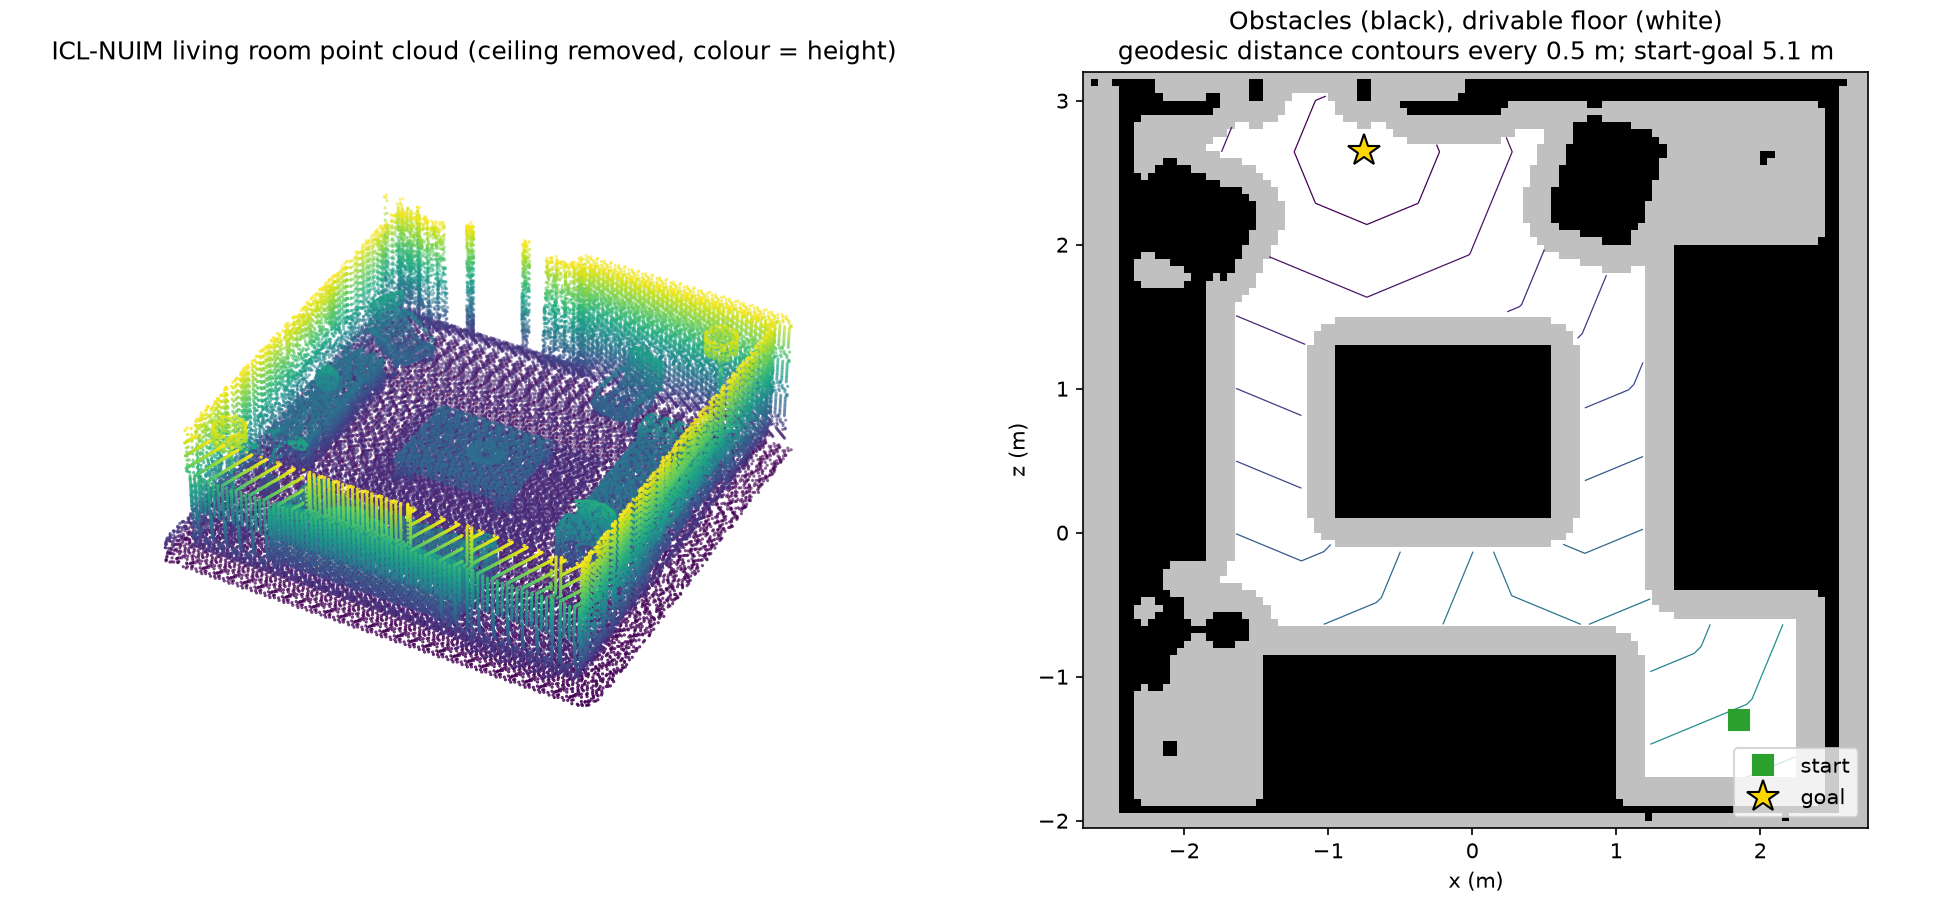
\includegraphics[width=\linewidth]{figures/livingroom_map.png}
\caption{Left: the room's point cloud. Right: the navigation map derived from it. Grey cells are
floor that the agent's centre cannot reach without touching an obstacle. Contours show the
geodesic distance to the goal (star), which defines progress and milestones.}
\label{fig:scene}
\end{figure}

\subsection{Agent and sensing}

The agent moves forward at a constant $v=\SI{0.2}{\metre\per\second}$; the culture chooses only
its turn rate $\omega$. At each \SI{10}{\milli\second} tick, $\theta\leftarrow\theta+\omega\,\Delta t$
and the position advances by $v\,\Delta t$ along $\theta$. A step that would put the centre
outside the drivable grid is a collision. Eight rays are cast at
$\theta+22.5^\circ+45^\circ k$, $k=0,\dots,7$, so that rays 0--3 sweep the left side from front
to back and rays 4--7 sweep the right side from back to front. Each ray is marched in
\SI{2.5}{\centi\metre} steps until it reaches an obstacle cell or the maximum range
$d_{\max}=\SI{2}{\metre}$. There is deliberately no ray straight ahead, so every ray belongs
unambiguously to the left or the right half of the field of view.

\subsection{Electrode layout}

\begin{figure}[t]
\centering
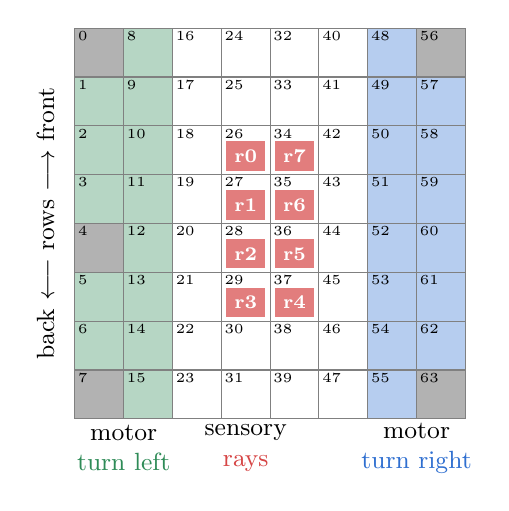
\begin{tikzpicture}[scale=0.62]
  \foreach \c in {0,...,7} \foreach \r in {0,...,7} {
    \pgfmathtruncatemacro{\ch}{8*\c+\r}
    \def\fillc{white}
    \ifnum\c<2 \def\fillc{motl!35}\fi
    \ifnum\c>5 \def\fillc{motr!35}\fi
    \ifnum\ch=0 \def\fillc{gray!60}\fi \ifnum\ch=7 \def\fillc{gray!60}\fi
    \ifnum\ch=56 \def\fillc{gray!60}\fi \ifnum\ch=63 \def\fillc{gray!60}\fi \ifnum\ch=4 \def\fillc{gray!60}\fi
    \fill[\fillc] (\c,-\r) rectangle ++(1,-1);
    \draw[gray] (\c,-\r) rectangle ++(1,-1);
    \node[font=\tiny, anchor=north west, inner sep=1pt] at (\c,-\r) {\ch};
  }
  \foreach \k/\c/\r in {0/3/2,1/3/3,2/3/4,3/3/5,4/4/5,5/4/4,6/4/3,7/4/2} {
    \fill[sens!70] (\c+0.1,-\r-0.32) rectangle ++(0.8,-0.6);
    \node[font=\scriptsize\bfseries, text=white] at (\c+0.5,-\r-0.62) {r\k};
  }
  \node[font=\small, align=center] at (1,-8.6) {motor\\ \textcolor{motl}{turn left}};
  \node[font=\small, align=center] at (3.5,-8.6) {sensory\\ \textcolor{sens}{rays}};
  \node[font=\small, align=center] at (7,-8.6) {motor\\ \textcolor{motr}{turn right}};
  \node[font=\small, rotate=90] at (-0.6,-4) {back $\longleftarrow$ rows $\longrightarrow$ front};
\end{tikzpicture}
\caption{Channel layout on the CL1's $8\times8$ array (channel $=8\cdot\text{column}+\text{row}$).
Grey channels are unusable: the four grounded corners and the reference channel~4. The sensory
strip is a coarse top-down map of the agent's view, with left rays in column~3 and right rays in
column~4. Columns 2 and 5 are a buffer that keeps stimulation artifacts and direct evoked responses
away from the 13 left and 14 right motor electrodes.}
\label{fig:layout}
\end{figure}

Figure~\ref{fig:layout} shows the layout. Like DishBrain, it uses eight sensory electrodes and
two counterbalanced motor regions. The motor regions sit at opposite edges, as far as possible
from the stimulated electrodes, so that most of what they record should come from activity
travelling through the culture. The placement implies a topographic prior: obstacles on the
left stimulate the left half of the sensory strip, which is closer to the left motor region. If
activity spreads locally, this alone could push the agent \emph{towards} obstacles. The mirrored
condition (Section~\ref{sec:design}) controls for this kind of wiring effect.

\subsection{Sensory encoding}

Each ray's distance is converted into a pulse rate on its own electrode, as in the rate code
DishBrain used for ball distance:
\begin{equation}
  f_k = f_{\min} + (f_{\max}-f_{\min})\left(1-\min\!\left(d_k/d_{\max},\,1\right)\right),\qquad
  f_{\min}=\SI{4}{\hertz},\ f_{\max}=\SI{40}{\hertz}.
\end{equation}
Pulses are timed by one phase accumulator per electrode: $\phi_k\mathrel{+}=f_k\Delta t$, and a
pulse is due when $\phi_k\geq1$. The accumulators start at random phases so that the electrodes
do not fire in lockstep. All pulses due in a tick go out in one \code{neurons.stim(ChannelSet(\dots),
StimDesign(160,-1.0,160,1.0))} call: a charge-balanced biphasic pulse,
\SI{160}{\micro\second} per phase at \SI{1}{\micro\ampere}, negative phase first. DishBrain
specified its stimulation in millivolts on a different array, so these currents are a starting
point to confirm with the CL1 team, not a translation.

\subsection{Motor decoding}

At each tick, the spikes detected on the two motor regions are counted and smoothed into rates
$r_L, r_R$ with a \SI{100}{\milli\second} exponential moving average. Each rate is divided by its
own slow baseline $b_s$, a \SI{30}{\second} moving average of the rate. The turn rate is then set
by the lateralisation index of the normalised rates:
\begin{equation}
  \tilde r_s = \frac{r_s}{b_s},\qquad
  \omega = \omega_{\max}\tanh\!\left(g\,\frac{\tilde r_L-\tilde r_R}{\tilde r_L+\tilde r_R}\right),\qquad
  \omega_{\max}=\SI{1.5}{\radian\per\second},\ g=6.
\end{equation}
The baseline removes each region's own bias, so a region that is simply more active does not
steer the agent. The index makes the turn rate depend only on how activity is split between
the regions, not on its overall level.

This second step matters. An earlier version used the plain difference
$\tilde r_L-\tilde r_R$. When sensory stimulation started after calibration, both regions sped
up several-fold, the difference saturated, and the agent turned at full rate for the first
minute or so, until the baselines caught up. The resulting improvement over episodes was
statistically significant ($\rho=0.54$, $p=0.002$) on a toy culture with no plasticity at all.
Analysed naively, it would have looked like learning. Before the first episode
there is a \SI{10}{\second} calibration period without stimulation, which fills the baselines.
The session stops with an error if either motor region is silent during calibration, because
the electrodes would then need to be moved to active areas of the culture.

\subsection{Feedback and episodes}

\begin{table}[t]
\centering\small
\begin{tabular}{@{}p{3.6cm}p{5.4cm}p{2.4cm}p{2cm}@{}}
\toprule
event & \code{feedback} condition & \code{silent} / \code{rest} & then \\
\midrule
milestone (\SI{0.5}{\metre} of new geodesic progress) & predictable: all 8 sensory, 10 pulses @ \SI{100}{\hertz} & \SI{100}{\milli\second} pause & continue \\
goal (within \SI{0.3}{\metre}) & predictable (as above) & \SI{100}{\milli\second} pause & new episode \\
collision & unpredictable: random sensory electrode, \SI{2}{\micro\ampere}, \SI{5}{\hertz} for \SI{4}{\second} & \SI{4}{\second} pause & new episode \\
timeout (\SI{60}{\second}) & none & none & new episode \\
\bottomrule
\end{tabular}
\caption{Events and their consequences. During feedback and pauses the agent is frozen and no
sensory pulses are sent, so feedback replaces sensory input as in DishBrain.}
\label{tab:feedback}
\end{table}

Table~\ref{tab:feedback} lists the events. The feedback parameters follow DishBrain: a
\SI{100}{\milli\second}, \SI{100}{\hertz} burst on all sensory electrodes after a hit, and
\SI{4}{\second} of \SI{5}{\hertz} pulses at random sensory sites, at twice the hit amplitude,
after a miss~\citep{kagan2022dishbrain,khajehnejad2024sample}. Pong produces a hit every few
seconds, but reaching the goal is rare early on, so progress milestones provide denser
predictable feedback. A milestone fires each time the geodesic distance to the goal drops
\SI{0.5}{\metre} below the best value reached so far in the episode. This rewards new progress
only, not driving back and forth.

The culture is never told where the goal is. The rays carry only obstacle information, so a
culture can learn to avoid collisions from the rays alone. Heading for the goal requires
learning a route from feedback alone, which is much harder. Adding an explicit goal-bearing input
is the first extension on the to-do list.

\subsection{Experimental design}\label{sec:design}

Three conditions follow the DishBrain controls:
\begin{description}[nosep, font=\normalfont\ttfamily]
  \item[feedback] sensory stimulation plus predictable and unpredictable feedback;
  \item[silent] sensory stimulation, with each feedback period replaced by a silent pause of the
        same length. Any improvement here comes from the sensory input alone;
  \item[rest] no stimulation at all; spontaneous activity steers the agent. This measures what
        an unstimulated culture does in this room.
\end{description}
The \code{--mirror} flag swaps the motor regions. If behaviour comes from the layout's
topographic prior, it flips with the mirror. If it is learned from feedback, it should appear in
both orientations. The recommended unit is a 20-minute session, as in DishBrain. Conditions
should be counterbalanced in order across sessions and cultures, with at least three sessions
per condition before comparing conditions.

\subsection{Measurements and analysis}\label{sec:analysis}

Every tick is logged to a \code{nav} data stream: pose, rays, turn rate, motor rates and
delivered pulses. Every episode start and end is logged to an \code{events} data stream. Both
are stored in the CL HDF5 recording next to the spikes and stimulation events. \code{analyze.py}
reports:
\begin{itemize}[nosep]
  \item \textbf{progress} per episode, $1-D_{\text{end}}/D_{\text{start}}$ with $D$ the geodesic
        distance (1 at the goal), and the fraction of episodes ending at the goal, in a collision
        or in a timeout;
  \item \textbf{within-session learning}: the Spearman correlation between episode index and
        progress, and a one-sided Mann--Whitney test of the last third of episodes against the
        first third. DishBrain compared the first 5 minutes with the last 15;
  \item \textbf{between conditions}: two-sided Mann--Whitney tests on per-episode progress,
        pooled by condition. Episodes within a session are not independent, so these $p$-values
        are optimistic; a session-level or mixed-effects analysis is on the to-do list;
  \item \textbf{steering coupling}: the correlation, over all ticks of play, between how much
        closer the obstacles are on the left than on the right ($\sum_{k<4}c_k-\sum_{k\geq4}c_k$
        with closeness $c_k=1-\min(d_k/d_{\max},1)$) and the decoded turn rate. Negative means the
        agent turns away from obstacles, positive means it turns towards them, and near zero means
        motor output ignores the sensory input;
  \item \textbf{motor PSTH}: the firing rate of the motor electrodes from \SIrange{-20}{30}{\milli\second}
        around each sensory pulse, in \SI{1}{\milli\second} bins. A sharp peak in the first
        \SI{2}{\milli\second} indicates a stimulation artifact rather than a neural response. This
        should be checked before interpreting any steering. Because pulses are issued on the
        \SI{10}{\milli\second} tick grid, dense stimulation produces a periodic PSTH; a short
        session with sparse pulses gives a cleaner picture.
\end{itemize}

\subsection{Implementation}

The loop runs at \SI{100}{\hertz} with \code{neurons.loop(100)}. Each tick casts the rays
(vectorised NumPy, well under a millisecond), updates the decoder and state machine, issues at
most one \code{stim} call, and appends one data-stream entry. On the CL1, the loop raises an
error if a tick overruns, and the code relies on that rather than recovering silently. The
simulator does not enforce this check (cl-sdk 1.0.0 prints a warning that jitter detection is
unsupported), so timing problems will only show up on the device. \code{prepare\_scene.py} runs
once on a laptop. Only \code{scene/livingroom.npz} (13\,kB) needs copying to the CL1, which needs
just \code{numpy} and \code{cl} to run \code{run.py}. Passing \code{live\_view=True} to
\code{run\_session} shows a top-down view of the room next to the electrode array in Jupyter
(Figure~\ref{fig:live}).

\begin{figure}[t]
\centering
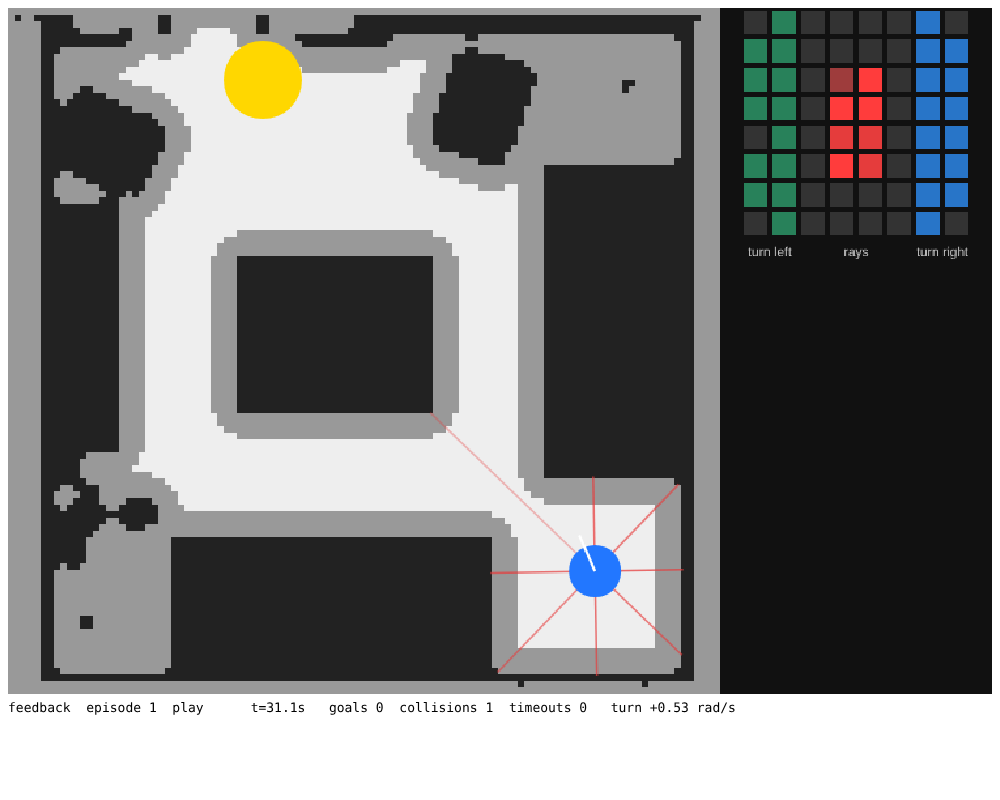
\includegraphics[width=0.82\linewidth]{figures/live_view.png}
\caption{The live view during a simulator session. The agent (blue) faces the white tick; red
rays are brighter when an obstacle is closer, the green line is the current episode's path,
and the yellow disc is the goal. On the array panel, sensory electrodes flash when pulsed and
motor regions glow with their current rate.}
\label{fig:live}
\end{figure}

\subsection{Pipeline checks on the simulator}

The SDK's default random source fires spontaneously but ignores stimulation. On that source, a
correct pipeline and a broken one look the same. \code{culture.py} replaces it with a toy culture
that adds evoked spikes on top of the random background:
\begin{itemize}[nosep]
  \item \textbf{local}: each pulse makes electrodes within 1.5 pitches fire with probability
        0.4 (scaled by current), 2--\SI{10}{\milli\second} later. These responses never reach
        the motor regions, so this is the negative control;
  \item \textbf{avoider}: in addition, each left-ray electrode drives every right-motor electrode
        (and vice versa) with probability 0.5, 5--\SI{20}{\milli\second} later. This is a
        Braitenberg vehicle~\citep{braitenberg1984vehicles} that turns away from close
        obstacles. It is a positive control: if the encoder, layout, decoder and sign
        conventions are right, it must avoid walls.
\end{itemize}
The toy culture has no plasticity, so no learning is expected, and none should be detected.

\begin{table}[t]
\centering\small
\begin{tabular}{@{}lrrrrrrrr@{}}
\toprule
session & episodes & goal & collision & progress & first & last & $\rho$ ($p$) & coupling \\
\midrule
\code{feedback}, avoider          & 31 & 0.00 & 1.00 & 0.48 & 0.53 & 0.48 & $-0.20$ (0.28) & $-0.50$ \\
\code{feedback --mirror}, avoider & 31 & 0.00 & 1.00 & 0.42 & 0.50 & 0.41 & $-0.07$ (0.72) & $-0.51$ \\
\code{feedback}, local            & 69 & 0.00 & 1.00 & 0.08 & 0.09 & 0.08 & $0.01$ (0.95)  & $-0.04$ \\
\code{rest}, local                & 71 & 0.00 & 1.00 & 0.07 & 0.08 & 0.08 & $0.04$ (0.74)  & $-0.03$ \\
\bottomrule
\end{tabular}
\caption{Four 10-minute sessions on the simulator (accelerated time, seed 7). ``first'' and
``last'' are the mean progress of the first and last third of episodes; $\rho$ is the Spearman
correlation of progress with episode index; ``coupling'' is the steering coupling defined in
Section~\ref{sec:analysis}.}
\label{tab:sim}
\end{table}

\begin{figure}[t]
\centering
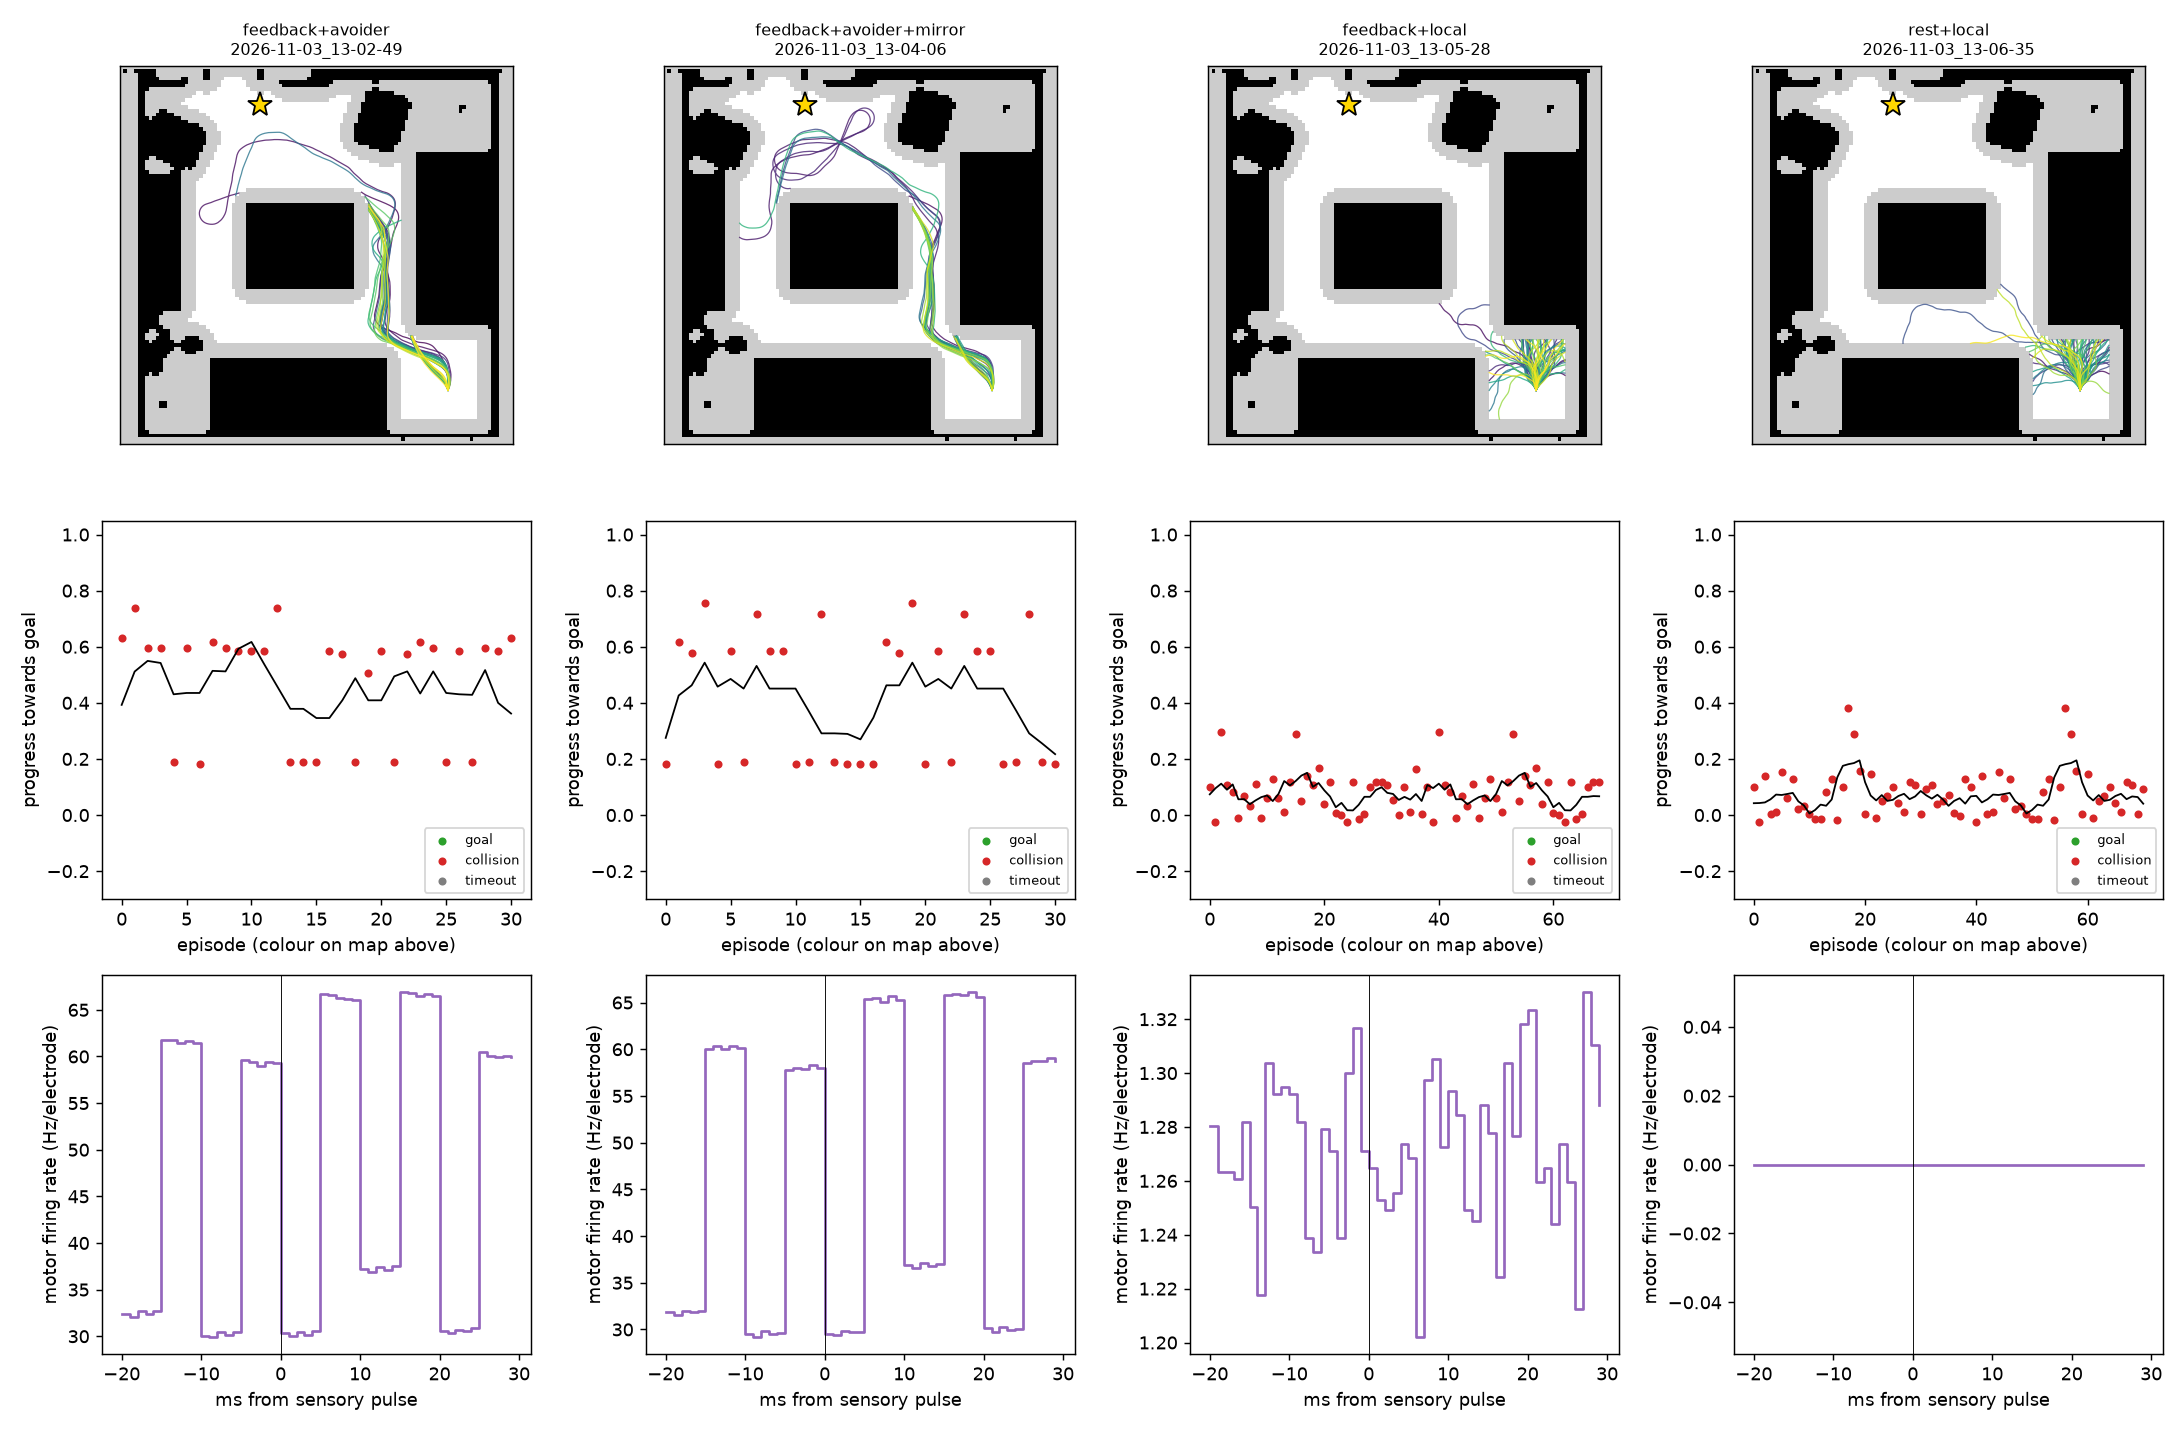
\includegraphics[width=\linewidth]{figures/sessions.png}
\caption{Output of \code{analyze.py} for the simulator sessions in Table~\ref{tab:sim}. Top:
trajectories coloured by episode. Middle: progress per episode, coloured by outcome, with a
5-episode running mean. Bottom: motor PSTH around sensory pulses. For the avoider, the
alternating bands come from dense pulses on the 10\,ms tick grid combined with the toy's
5--20\,ms response latency. For the local toy culture, motor rates stay at the spontaneous
level of about 1.3\,Hz. The rest condition sends no pulses, so its PSTH is empty.}
\label{fig:sessions}
\end{figure}

Table~\ref{tab:sim} and Figure~\ref{fig:sessions} show the expected pattern. The avoider turns
away from obstacles (coupling $-0.50$). It leaves the alcove, follows the right-hand corridor
north and usually collides where the corridor opens out at the top of the map, about halfway along
the route. That is about six times as far as the local toy culture
(0.48 vs 0.08 progress, $p<10^{-13}$). The local toy culture and the rest condition do not
differ ($p=0.61$), and neither shows any coupling. This shows that sensory pulses that never
reach the motor regions are equivalent to no input at all. The mirrored avoider still avoids,
because its wiring was built against the decoded layout. Most importantly, no session shows a
significant trend over episodes, which is correct for a culture with no plasticity. On real
cells, the avoider's numbers are a rough upper reference for what pure reflexive avoidance can
achieve in this room, and the local and rest sessions show what chance looks like. None of
these simulator sessions reached the goal: reflexes alone do not find the far corner.

\section{To-do list}

\subsection*{Before the event}
\begin{itemize}[leftmargin=2em]
  \done Scene converter, closed loop, toy culture, analysis and live view; pipeline checks
        on the simulator (Table~\ref{tab:sim}).
  \todo Set up a Python~3.12+ environment on the laptop, \code{pip install -r requirements.txt},
        run \code{prepare\_scene.py}, and repeat the \code{--toy avoider} and \code{--toy local}
        runs to confirm everything works on the laptop.
  \todo Questions for the Callosum / Frontier Computing team: how code reaches the CL1
        (Jupyter on the device?), which cell type is plated and how old the culture is, sensible
        stimulation currents (the \SI{1}{\micro\ampere} and \SI{2}{\micro\ampere} defaults are guesses),
        and how many minutes of device time each team gets.
  \todo Re-read the DishBrain methods~\citep{kagan2022dishbrain}, especially the sensory and motor
        region placement and the rest periods between rallies.
  \todo Prepare a one-slide pitch: the loop diagram (Figure~\ref{fig:loop}), the room
        (Figure~\ref{fig:scene}) and a recording of the live view.
\end{itemize}

\subsection*{At the event (limited CL1 time)}
\begin{itemize}[leftmargin=2em]
  \todo Copy the repository and \code{scene/livingroom.npz} to the device; no download is needed there.
  \todo Sanity check as in \code{CL-00 Hello, Neurons}: pulse one sensory electrode and confirm a response
        in the visualiser.
  \todo Look at spontaneous activity across the array. If a motor region is quiet, move
        \code{MOTOR\_LEFT} and \code{MOTOR\_RIGHT} (and if needed \code{SENSORY}) in \code{config.py}
        to active areas, keeping the buffer columns between them.
  \todo Run a 2-minute \code{rest} session and a 2-minute \code{feedback} session and check the
        motor PSTH. An early peak means an artifact: lower the current, widen the buffer, or
        ignore motor spikes within \SI{2}{\milli\second} of a pulse.
  \todo Run one \code{feedback} session (10--20 min) with the live view, then one \code{rest}
        session as a baseline, and run \code{analyze.py} on both.
  \todo Record the screen of the live view for the pitch.
\end{itemize}

\subsection*{If there is a day on the CL1}
\begin{itemize}[leftmargin=2em]
  \todo Full design: \code{feedback}, \code{silent}, \code{rest}, each at least three 20-minute
        sessions, counterbalanced, plus \code{feedback --mirror}; more than one culture if possible.
  \todo Any change to the decoder or the feedback should first be run on \code{--toy avoider}
        and \code{--toy local} for the session length used on the cells. Any trend across
        episodes on the toy culture is an artifact of the pipeline, not learning (see the
        decoding section).
  \todo Replace pooled episode tests with session-level statistics (one value per session) or a
        mixed-effects model with episodes nested in sessions nested in cultures.
  \todo Retention: repeat a \code{feedback} session after 45--60 minutes of rest, since
        \citet{robbins2026organoids} found the improvement faded.
  \todo Software baselines with the same number of episodes: a random-turn agent, a hand-wired
        Braitenberg avoider, and a small RL agent~\citep{khajehnejad2024sample}.
\end{itemize}

\subsection*{Extensions}
\begin{itemize}[leftmargin=2em]
  \todo \textbf{Goal bearing.} Add one or two electrodes whose rate encodes the direction to the
        goal (or to the next waypoint on the geodesic path). Without this input the culture can
        only learn to avoid obstacles.
  \todo \textbf{Curriculum.} Start episodes closer to the goal and move the start back as progress
        improves; shorter milestones early on.
  \todo \textbf{Adaptive training signal.} Choose which electrodes receive feedback with a
        bandit or RL algorithm, as in~\citet{robbins2026organoids}.
  \todo \textbf{Full 3D sensing.} Cast rays at several elevations directly against the point cloud
        (or a voxel grid) so that table tops and overhangs matter; try the Redwood office scenes or
        a maze.
  \todo \textbf{Richer decoding.} Use frequency content of the raw signal rather than spike counts,
        which worked better for digit classification~\citep{loeffler2026digits}; or choose motor
        regions per culture, as DishBrain did in pilot experiments.
  \todo \textbf{A plastic toy culture.} Add spike-timing-dependent plasticity to \code{culture.py}
        to test, on the simulator, whether this feedback scheme can shape behaviour at all.
\end{itemize}

\subsection*{Known limitations}
\begin{itemize}[leftmargin=2em, nosep]
  \item The toy culture has no plasticity; simulator checks validate the plumbing, not learning.
  \item Stimulation currents are not calibrated, and DishBrain's voltages do not translate
        directly to the CL1's current-controlled stimulation.
  \item In accelerated mode the simulator gives its data producer \SI{100}{\milli\second} per
        tick. On a busy two-core machine this occasionally raised
        \code{TimeoutError: Timeout waiting for timestamp}; rerunning with nothing else running
        fixed it.
\end{itemize}

\bibliographystyle{plainnat}
\bibliography{refs}
\end{document}
